\documentclass[12pt]{article}
\thispagestyle{empty}
\usepackage{amsmath}
\usepackage[margin=1in]{geometry}
\usepackage{amsfonts}
\usepackage{hyperref}
\usepackage{graphicx}
\usepackage{siunitx}
\usepackage{cancel}
\usepackage{xfrac}
\usepackage{listings}
\usepackage{longdivision}

\begin{document}
	
	\begin{center}
		\par\noindent \large \textbf{0.4 + 0.3 = 0.70000005?}  [ Andy Chong Sam ]
	\end{center}
	\begin{minipage}[t]{.5\linewidth}
		\par\noindent Floating point numbers are not exact representations of decimals  containing fractional amounts. For instance, in Java the code 0.3f + 0.4f produces the unusual result 0.70000005. On this article we'll try and derive this  result without necessarily taking a deep dive into hardware or Java implementation.
		\newline
		\par\noindent \textbf{(II)} A rounding system utilizing a (G)uard, (R)ound, and (S)ticky bit will be used. In this system, we'll assume that the least significant bit in the mantissa will be the guard bit. The round bit is the one after guard, and the sticky bit is the OR result of all remaining bits. Here are the rules:
		
		\begin{center}
			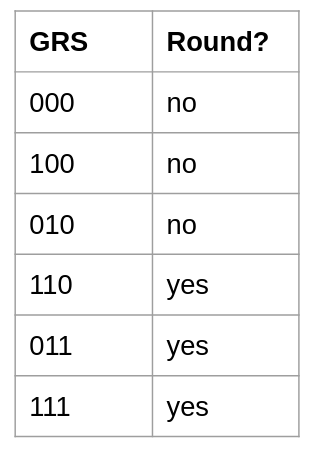
\includegraphics[width=3.4cm]{case-1.png}
		\end{center}
	
		\par\noindent \textbf{(III)} In binary, 0.4 is: \newline
		\(0\;\;01111101\;\;10011001100110011001101\) \newline
		\par\noindent The first cluster is 0, it's positive. For the exponent,\((01111101)_2 = (125)_{10}\).The mantissa to 27 bits, with bit 23 (G) in bold is:
		\begin{flalign*}
			1001100110011001100110\textbf{0}1100
		\end{flalign*}
		\par\noindent Using the rules from section II we round the mantissa to 23 bits:
		\begin{flalign*}
			10011001100110011001101
		\end{flalign*}
		\par\noindent In scientific notation, the stored float is:
		\begin{flalign*}
			1.10011001100110011001101 \times 2^{125}
		\end{flalign*}
	\end{minipage}	
	\hspace{0.45cm}
	\begin{minipage}[t]{.5\linewidth} 
		\textbf{(IV)} In binary, 0.3 is: \newline
		\(0\;\;01111101\;\;00110011001100110011010 \)\newline
		\par\noindent The exponent is 125, the mantissa shown up to 27 bits is, with the (G) bit in bold:
		\begin{flalign*}
		0011001100110011001100\textbf{1}1001
		\end{flalign*}
		\par\noindent Using the established rules we round this to:
		\begin{flalign*}
			00110011001100110011010
		\end{flalign*}
		\par\noindent Written in scientific notation:
		\begin{flalign*}
			1.0011001100110011001101 \times 2^{125}
		\end{flalign*}
	\par\noindent \textbf{(V)}The next step is to add the mantissas from steps III and IV together (along with the assumed 1), which is the result of 0.3f + 0.4f:
	\begin{flalign*}
		     1.10011001100110011001101 \\
		     + 1.00110011001100110011010\\
		     \rule{5cm}{0.1pt} \\
		     10.11001100110011001100111
	\end{flalign*}
	\par\noindent In scientific notation this result is: 
	\begin{flalign*}
	 10.11001100110011001100111 \times 2^{125} \\
		\text{After normalizing...} \\
	1.011001100110011001100111 \times 2^{126}
	\end{flalign*}
	\par\noindent Let's see how it's stored. The exponent is now \(01111110\), the binary representation of 126. We round based on the bolded (G) bit:
	\begin{flalign*}
		\text{0}\;\;\text{01111110}\;\;\text{0110011001100110011001\textbf{1}1}\\
		\text{0}\;\;\text{01111110}\;\;\text{0110011001100110011010}
	\end{flalign*}
	\par\noindent \textbf{(VI)} We use the formula \(	d = (-1)^s (1+m)\;2^e\) to verify the stored value. The calculation is shown in full on the next page but we find that this gives us approximately \textbf{0.700000048}... close enough!
	\end{minipage}
	\newpage
	\par\noindent  For the formula \(d = (-1)^s (1+m)\;2^e\)...
	\begin{itemize}
		\item \(s=0\) since the number is positive. 
		\item \(m\) is the decimal representation of the mantissa 0110011001100110011010
		\item  \(e = -1\). The value of e is derived by subtracting 127, the bias, from the exponent 126
	\end{itemize}
	\par\noindent Finally the calculation itself:
	\begin{flalign*}
		(-1)^0(1 + (2^{-2} + 2^{-3} + 2^{-6} + 2^{-7} + 2^{-10} + 2^{-11} + 2^{-14} + 2^{-15} + 2^{-18} + 2^{-19} + 2^{-21} ))(2^{-1}) \\
		\approx 0.700000048
	\end{flalign*}
	\par\noindent When rounded to include only six places after the decimal we get 0.70000005.
\end{document}